\section{Capacity-Data Regime Extension}

This secondary extension asks whether the observed behavior of expressive probe
heads changes with the amount of HBN training data. It reuses the frozen REVE
representation, preprocessing, external cohort, checkpoint rule, and training
contract of the primary study. The only planned factors are training size
($n\in\{200,400,800\}$), head family, and optimization seed. The matrix has
three heads, three training sizes, and ten seeds, for 90 frozen-head runs. The
external evaluation contains one prediction for every declared head-seed-subject
combination on the previously evaluated 75-subject primary cohort;
participant-level outputs are not included in this repository. The extension
does not add independent external subjects.

\subsection{Aggregate results}

The parameter counts are derived from the validated checkpoint metadata rather
than entered as manuscript constants. The aggregate external metrics and seed
variability are shown in Table~\ref{tab:capacity-absolute}. Paired candidate
contrasts against the training-size-matched mean-linear baseline are shown in
Table~\ref{tab:capacity-cells}. The six cell comparisons are positive for every
observed seed, but the uncertainty intervals are the primary indication of how
strongly those effects are supported.

\begin{table}[H]
  \centering
  \scriptsize
  \caption{Aggregate external Pearson performance in the capacity-data
  extension. Seed SD is computed across the ten matched optimization seeds.}
  \label{tab:capacity-absolute}
  \input{../results/extensions/capacity_data_regime_v3/capacity_data_regime_absolute.tex}
\end{table}

\begin{table}[H]
  \centering
  \scriptsize
  \caption{Paired candidate-baseline differences by training size. Intervals
  use the joint seed-subject bootstrap; Holm-adjusted p-values are exploratory
  and do not replace the primary sealed decision rule.}
  \label{tab:capacity-cells}
  \input{../results/extensions/capacity_data_regime_v3/capacity_data_regime_cells.tex}
\end{table}

The training-size contrasts quantify whether the candidate advantage itself
changes between nested training regimes. The endpoint and adjacent contrasts
are reported in Table~\ref{tab:capacity-contrasts}; none should be interpreted
as a universal scaling law. In particular, a larger training subset can change
both the baseline and candidate, so the relevant quantity is the paired change
in their difference, not the raw candidate score alone.

\begin{table}[H]
  \centering
  \scriptsize
  \caption{Exploratory changes in the paired candidate-baseline difference
  across training sizes.}
  \label{tab:capacity-contrasts}
  \input{../results/extensions/capacity_data_regime_v3/capacity_data_regime_contrasts.tex}
\end{table}

For context, the selected-head HBN validation scores and the corresponding
external scores are shown in Table~\ref{tab:capacity-transfer}. This is a
descriptive transfer view rather than a second selection criterion: the MIPDB
targets remain excluded from training and checkpoint selection.

\begin{table}[H]
  \centering
  \scriptsize
  \caption{Descriptive validation-to-external transfer for the candidate heads.}
  \label{tab:capacity-transfer}
  \input{../results/extensions/capacity_data_regime_v3/capacity_data_regime_validation_external_transfer.tex}
\end{table}

\subsection{Figures and robustness interpretation}

Figure~\ref{fig:capacity-absolute} displays the absolute external scores,
Figure~\ref{fig:capacity-delta} displays the paired deltas and bootstrap
intervals, and Figure~\ref{fig:capacity-seed-deltas} displays the per-seed
contrasts. The same 10,000-iteration hierarchical bootstrap is used throughout:
seeds and external subjects are resampled jointly while preserving candidate-
baseline pairing.

\begin{figure}[!ht]
  \centering
  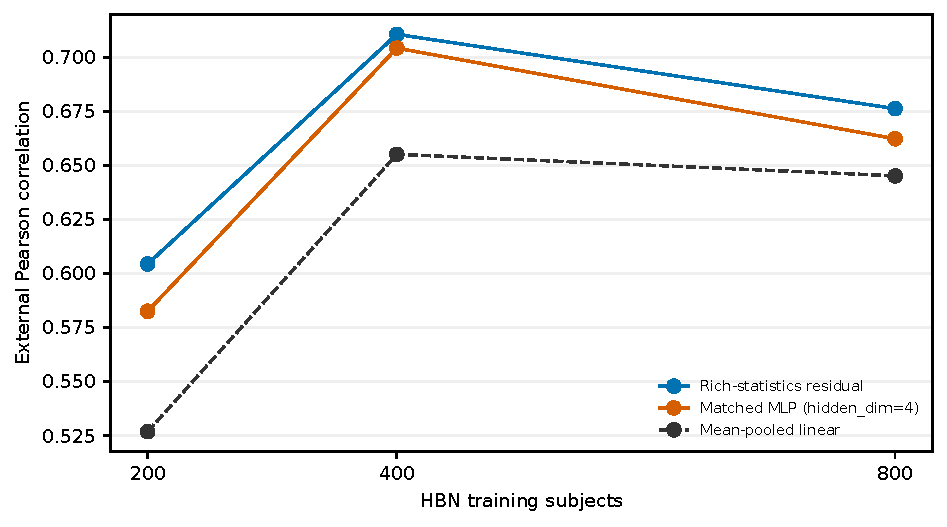
\includegraphics[width=0.94\linewidth]{../results/extensions/capacity_data_regime_v3/capacity_data_regime_absolute.pdf}
  \caption{Aggregate external Pearson scores across training sizes and probe
  heads.}
  \label{fig:capacity-absolute}
\end{figure}

\begin{figure}[!ht]
  \centering
  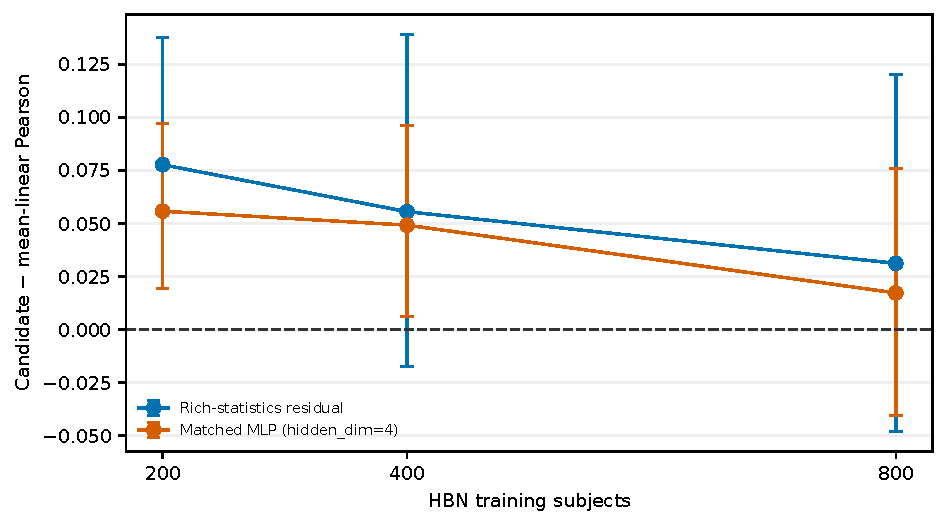
\includegraphics[width=0.94\linewidth]{../results/extensions/capacity_data_regime_v3/capacity_data_regime_delta.pdf}
  \caption{Paired external Pearson deltas relative to the matched mean-linear
  baseline, with joint bootstrap intervals.}
  \label{fig:capacity-delta}
\end{figure}

\begin{figure}[!ht]
  \centering
  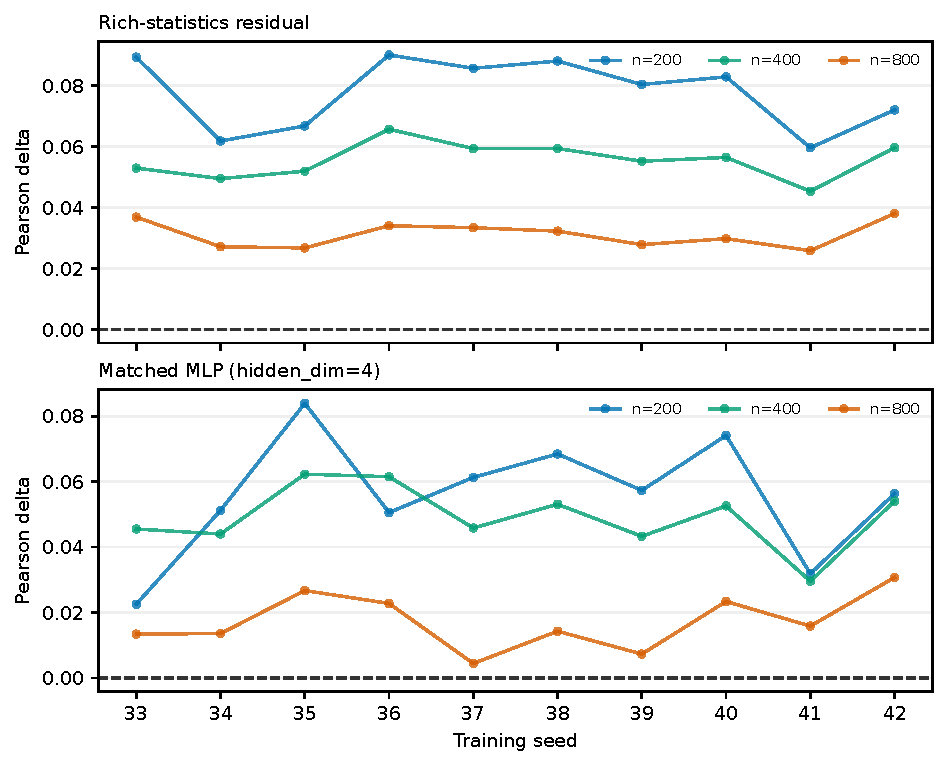
\includegraphics[width=0.94\linewidth]{../results/extensions/capacity_data_regime_v3/capacity_data_regime_seed_deltas.pdf}
  \caption{Seed-level paired external deltas for the two candidate heads.}
  \label{fig:capacity-seed-deltas}
\end{figure}

The exact seed sign-flip tests and Holm correction are exploratory descriptive
inference for this extension. Their configuration, family order, and canonical
digest are retained in the aggregate asset manifest. They do not alter the
primary predeclared superiority boundary: the sealed primary conclusion is
still determined by its hierarchical bootstrap, cohort, win-count, and
worst-seed criteria. The extension therefore supports a bounded statement
about head capacity under the tested data regimes, not a claim that a more
complex head is generally better or that additional training subjects have a
monotone effect.
